\subsection{Standard Signals}

\begin{figure}[h!]
\centering
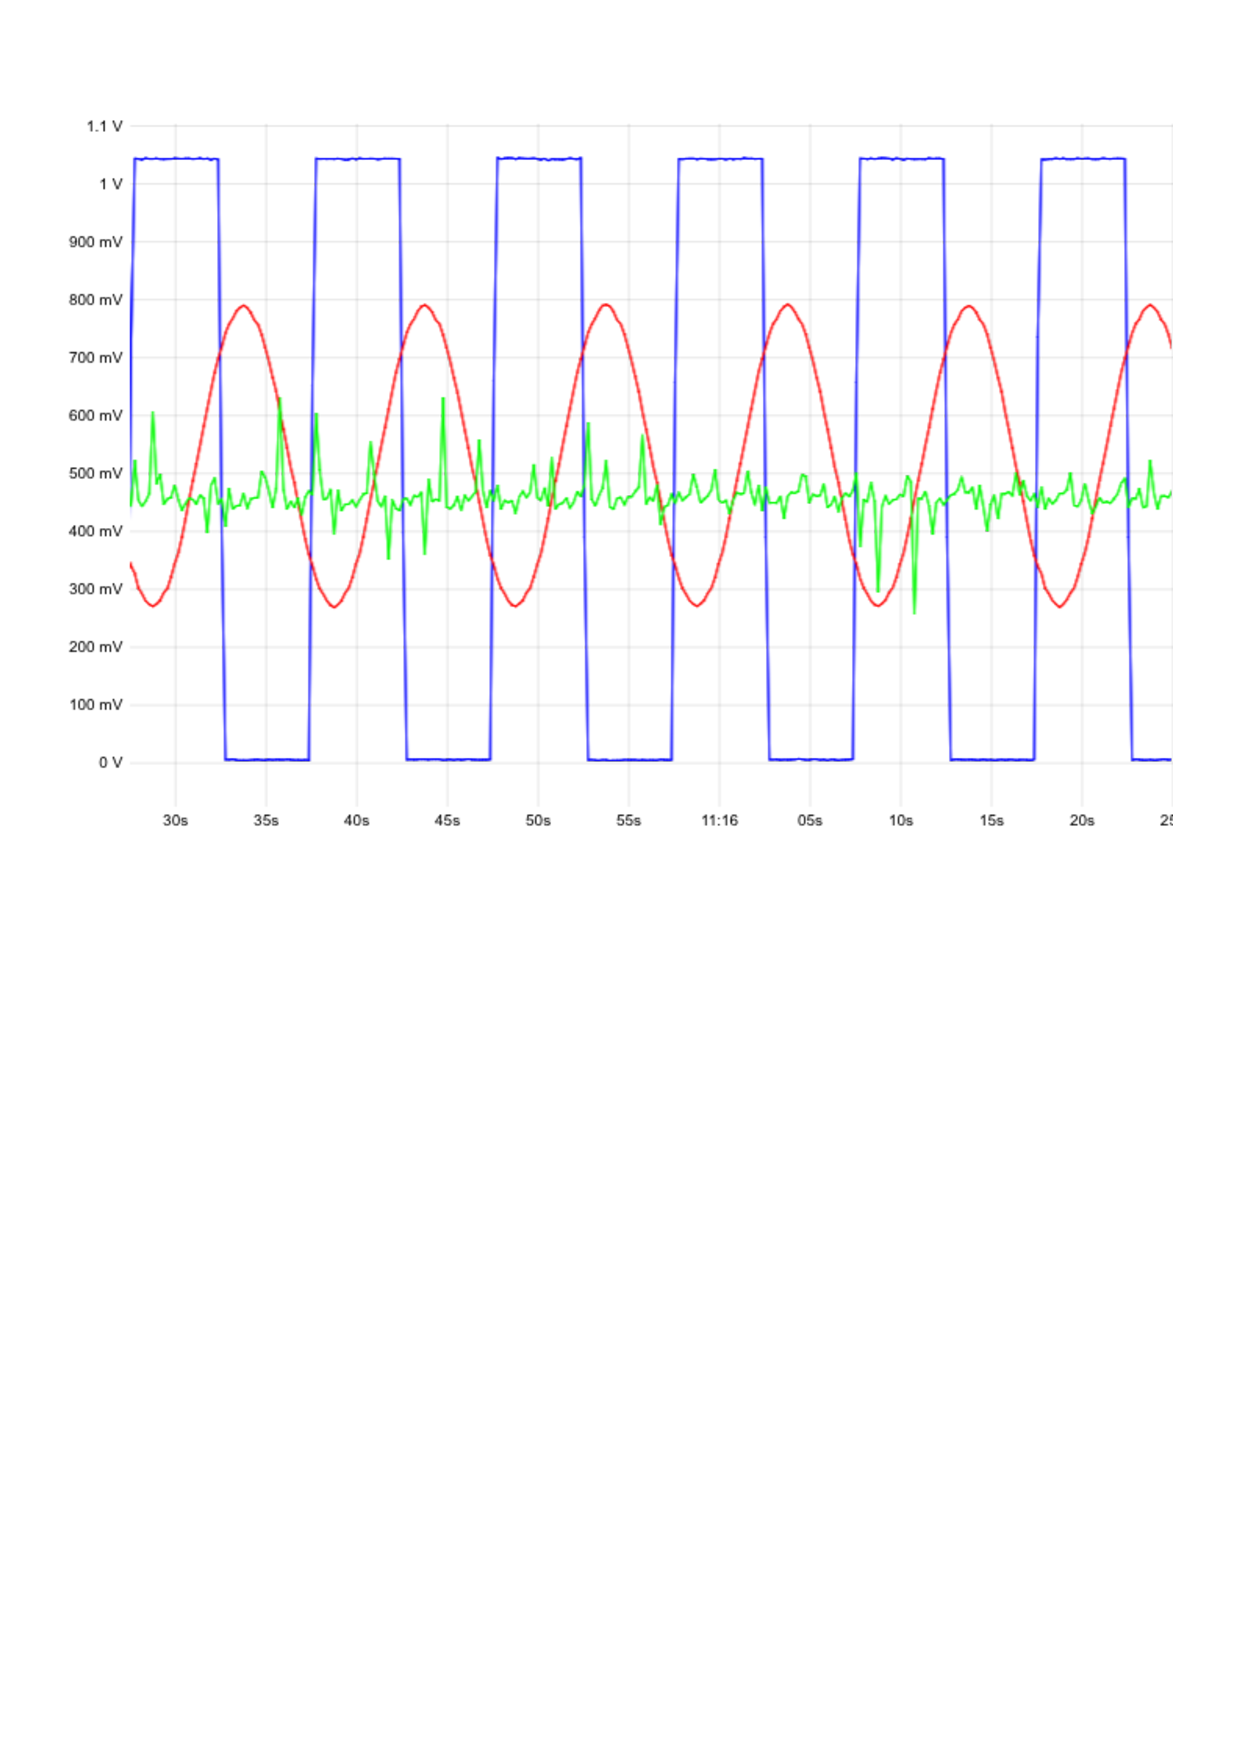
\includegraphics[trim={0cm 0cm 0cm  0cm}, clip, width=.75\textwidth]{./figures/standardsignals/picologChemComp.pdf}
\captionsetup{justification=centering}
\caption{Standard signals recorded using a PicoScope.}
\label{fig: test1 picolog}
\bigbreak
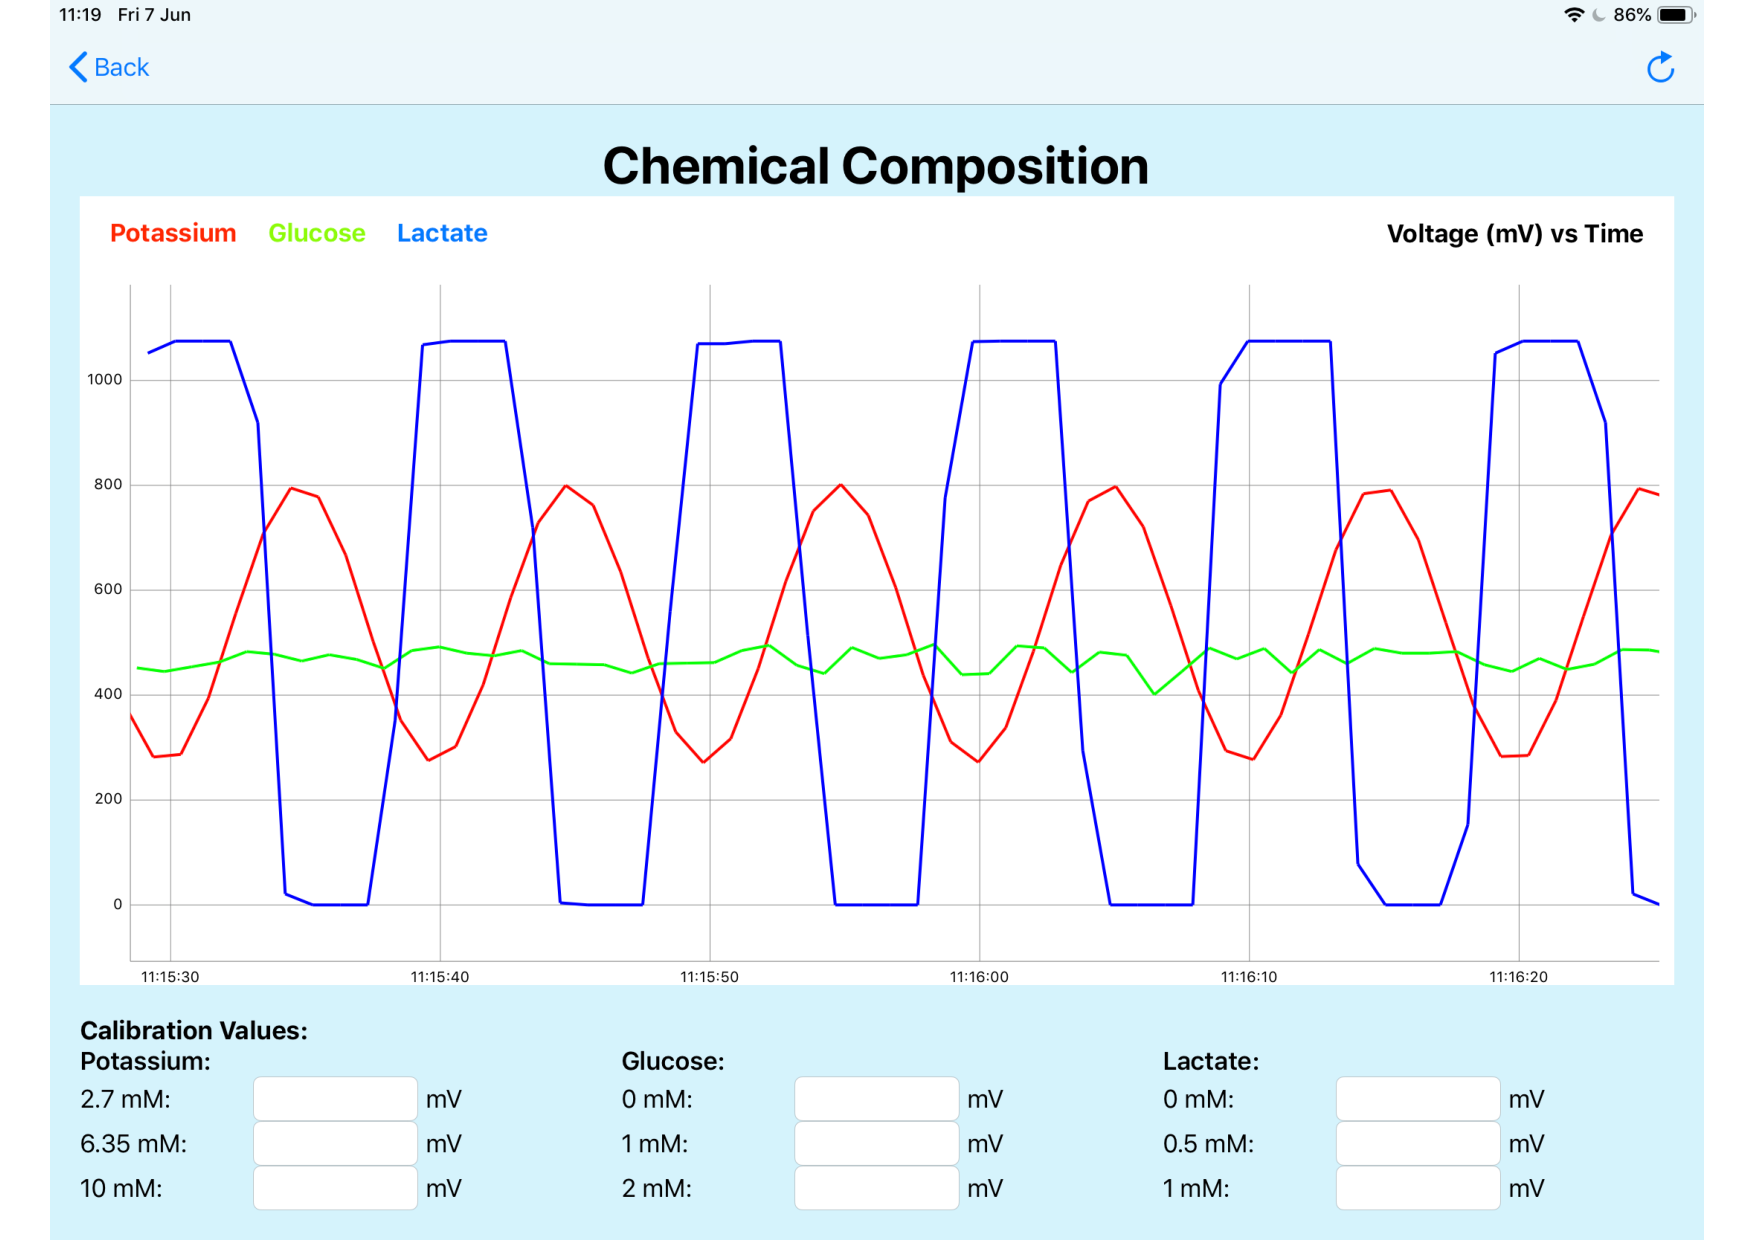
\includegraphics[trim={0cm 0cm 0cm  0cm}, clip, width=.75\textwidth]{./figures/standardsignals/appChemComp.pdf}
\captionsetup{justification=centering}
\caption{Standard signals recorded using the iPad app.}
\label{fig: test1 app}
\end{figure}



Figure~\ref{fig: test1 picolog} shows the raw signals received on PicoLog, and Figure~\ref{fig: test1 app} shows the three signals received on the Chemical Composition page of the app after undergoing filtering and processing on the Arduino. The noise signal is shown in green in both plots, the square wave in blue, and the sine wave in red.


\subsection{Spreading Depolarisation}

\begin{figure}[h!]
\centering
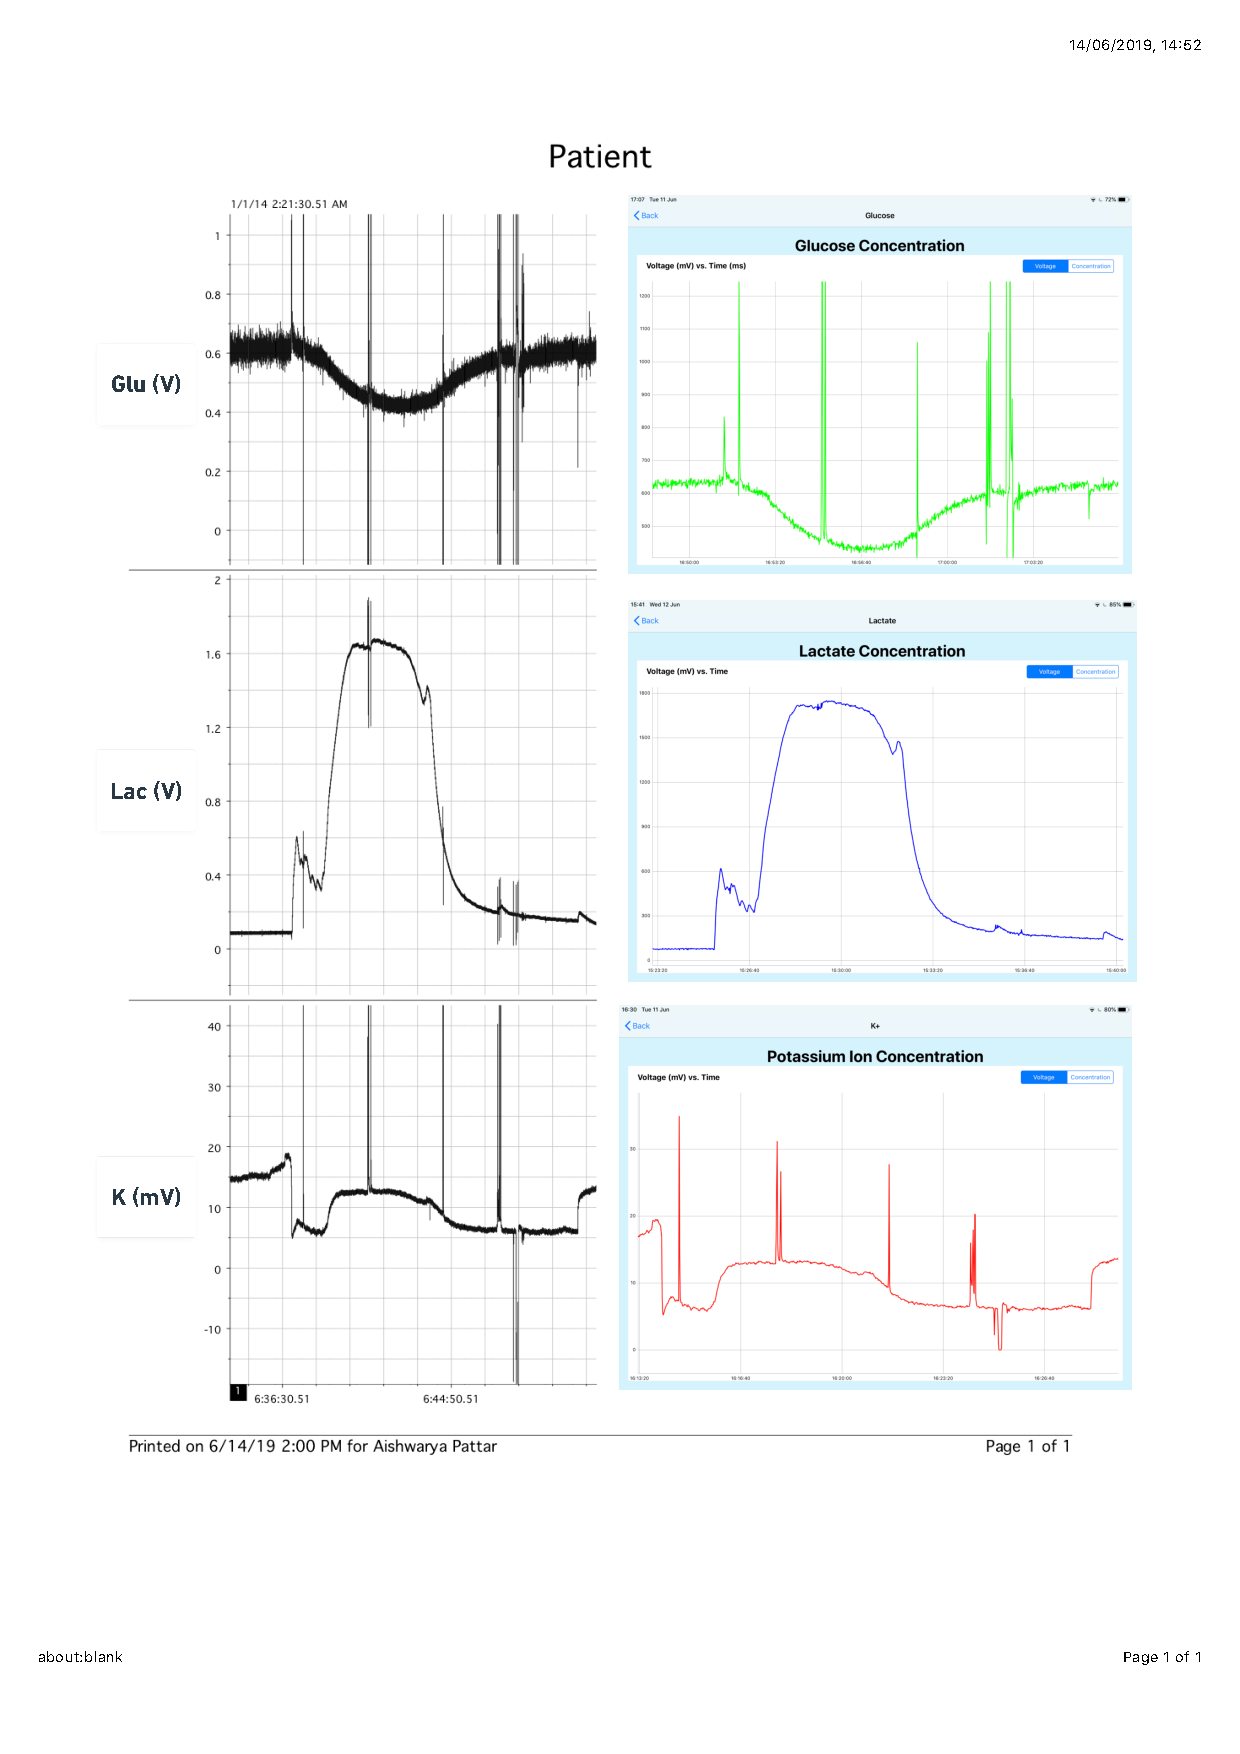
\includegraphics[trim={1.25cm 6cm 1.5cm  3cm}, clip, width=1\textwidth]{./figures/test2.pdf}
\captionsetup{justification=centering}
\caption{Left: Raw patient data obtained from LabChart. Right: Signals received on app. From top to bottom: Glucose, Lactate, Potassium.}
\label{fig: test2}
\end{figure}

Figure~\ref{fig: test2} shows the raw patient signals, before downsampling and processing, compared to the signal received on the app. Figure~\ref{fig: test2 conc} shows the concentration graphs produced on the app calculated from the inputted calibration values.

\begin{figure}[p]
\centering
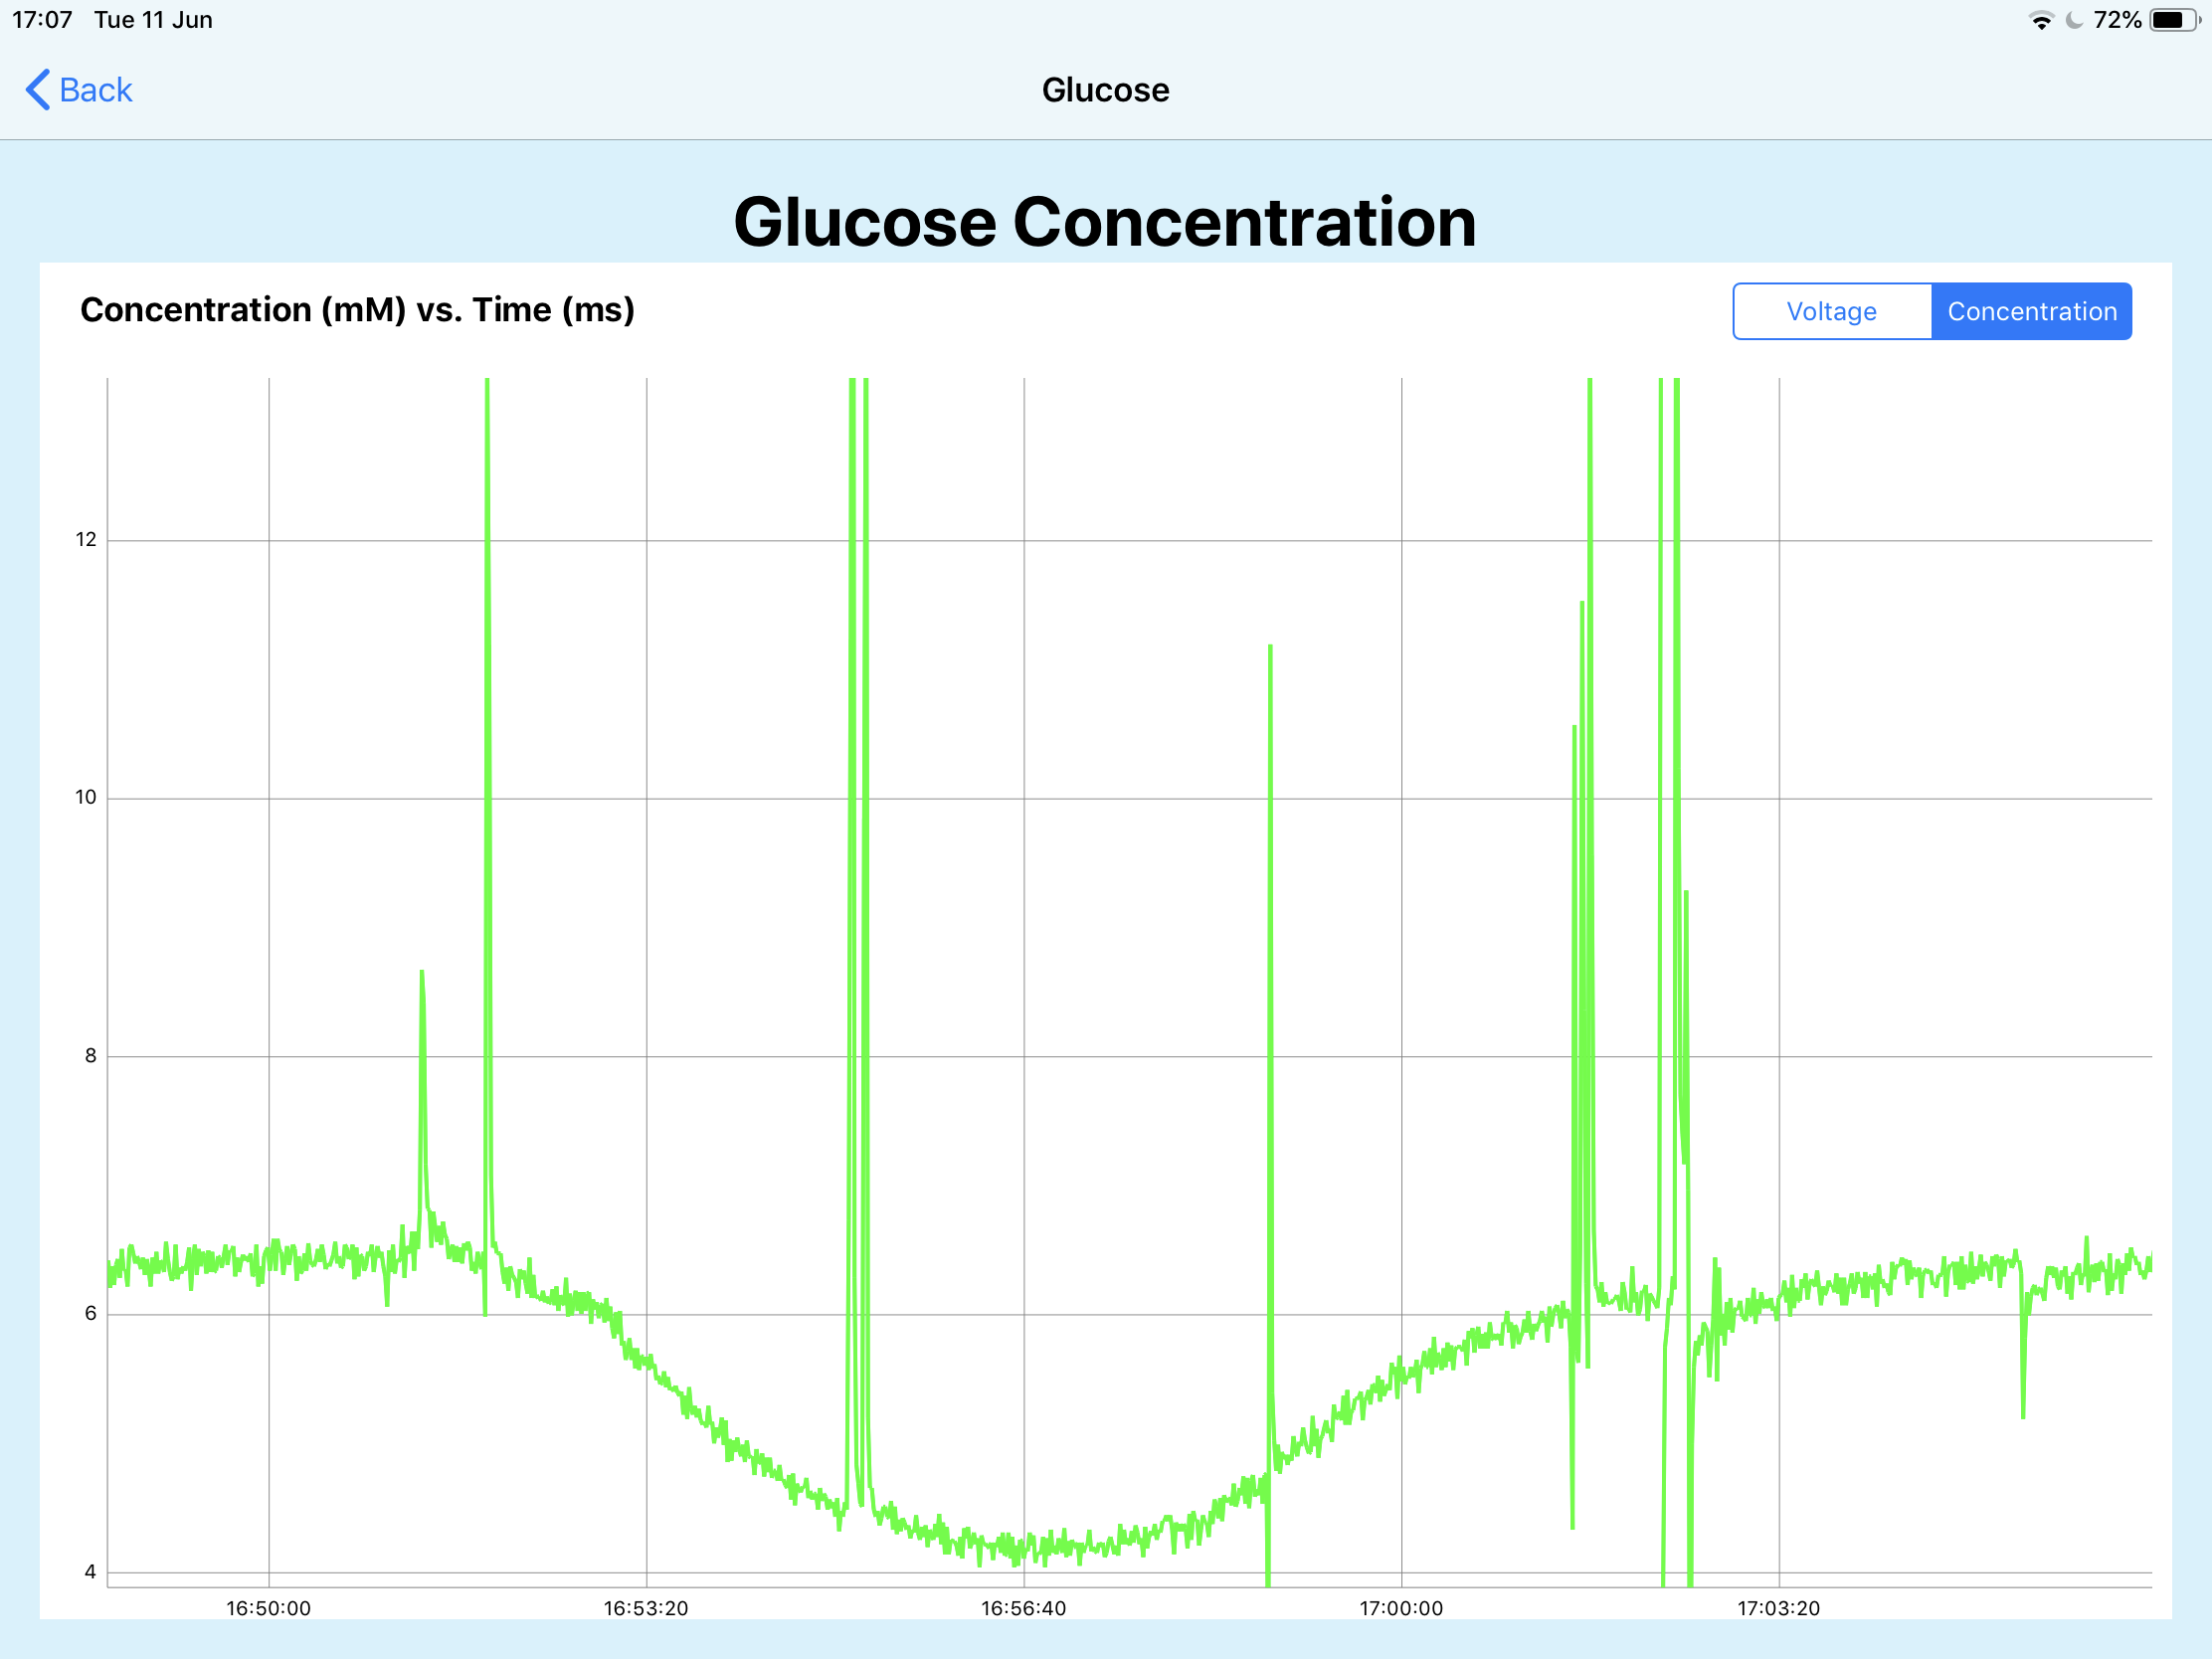
\includegraphics[trim={1.3cm 1.3cm 1.3cm  10cm}, clip, width=.75\textwidth]{./figures/patientsignals/GlucoseC.PNG}
\bigbreak
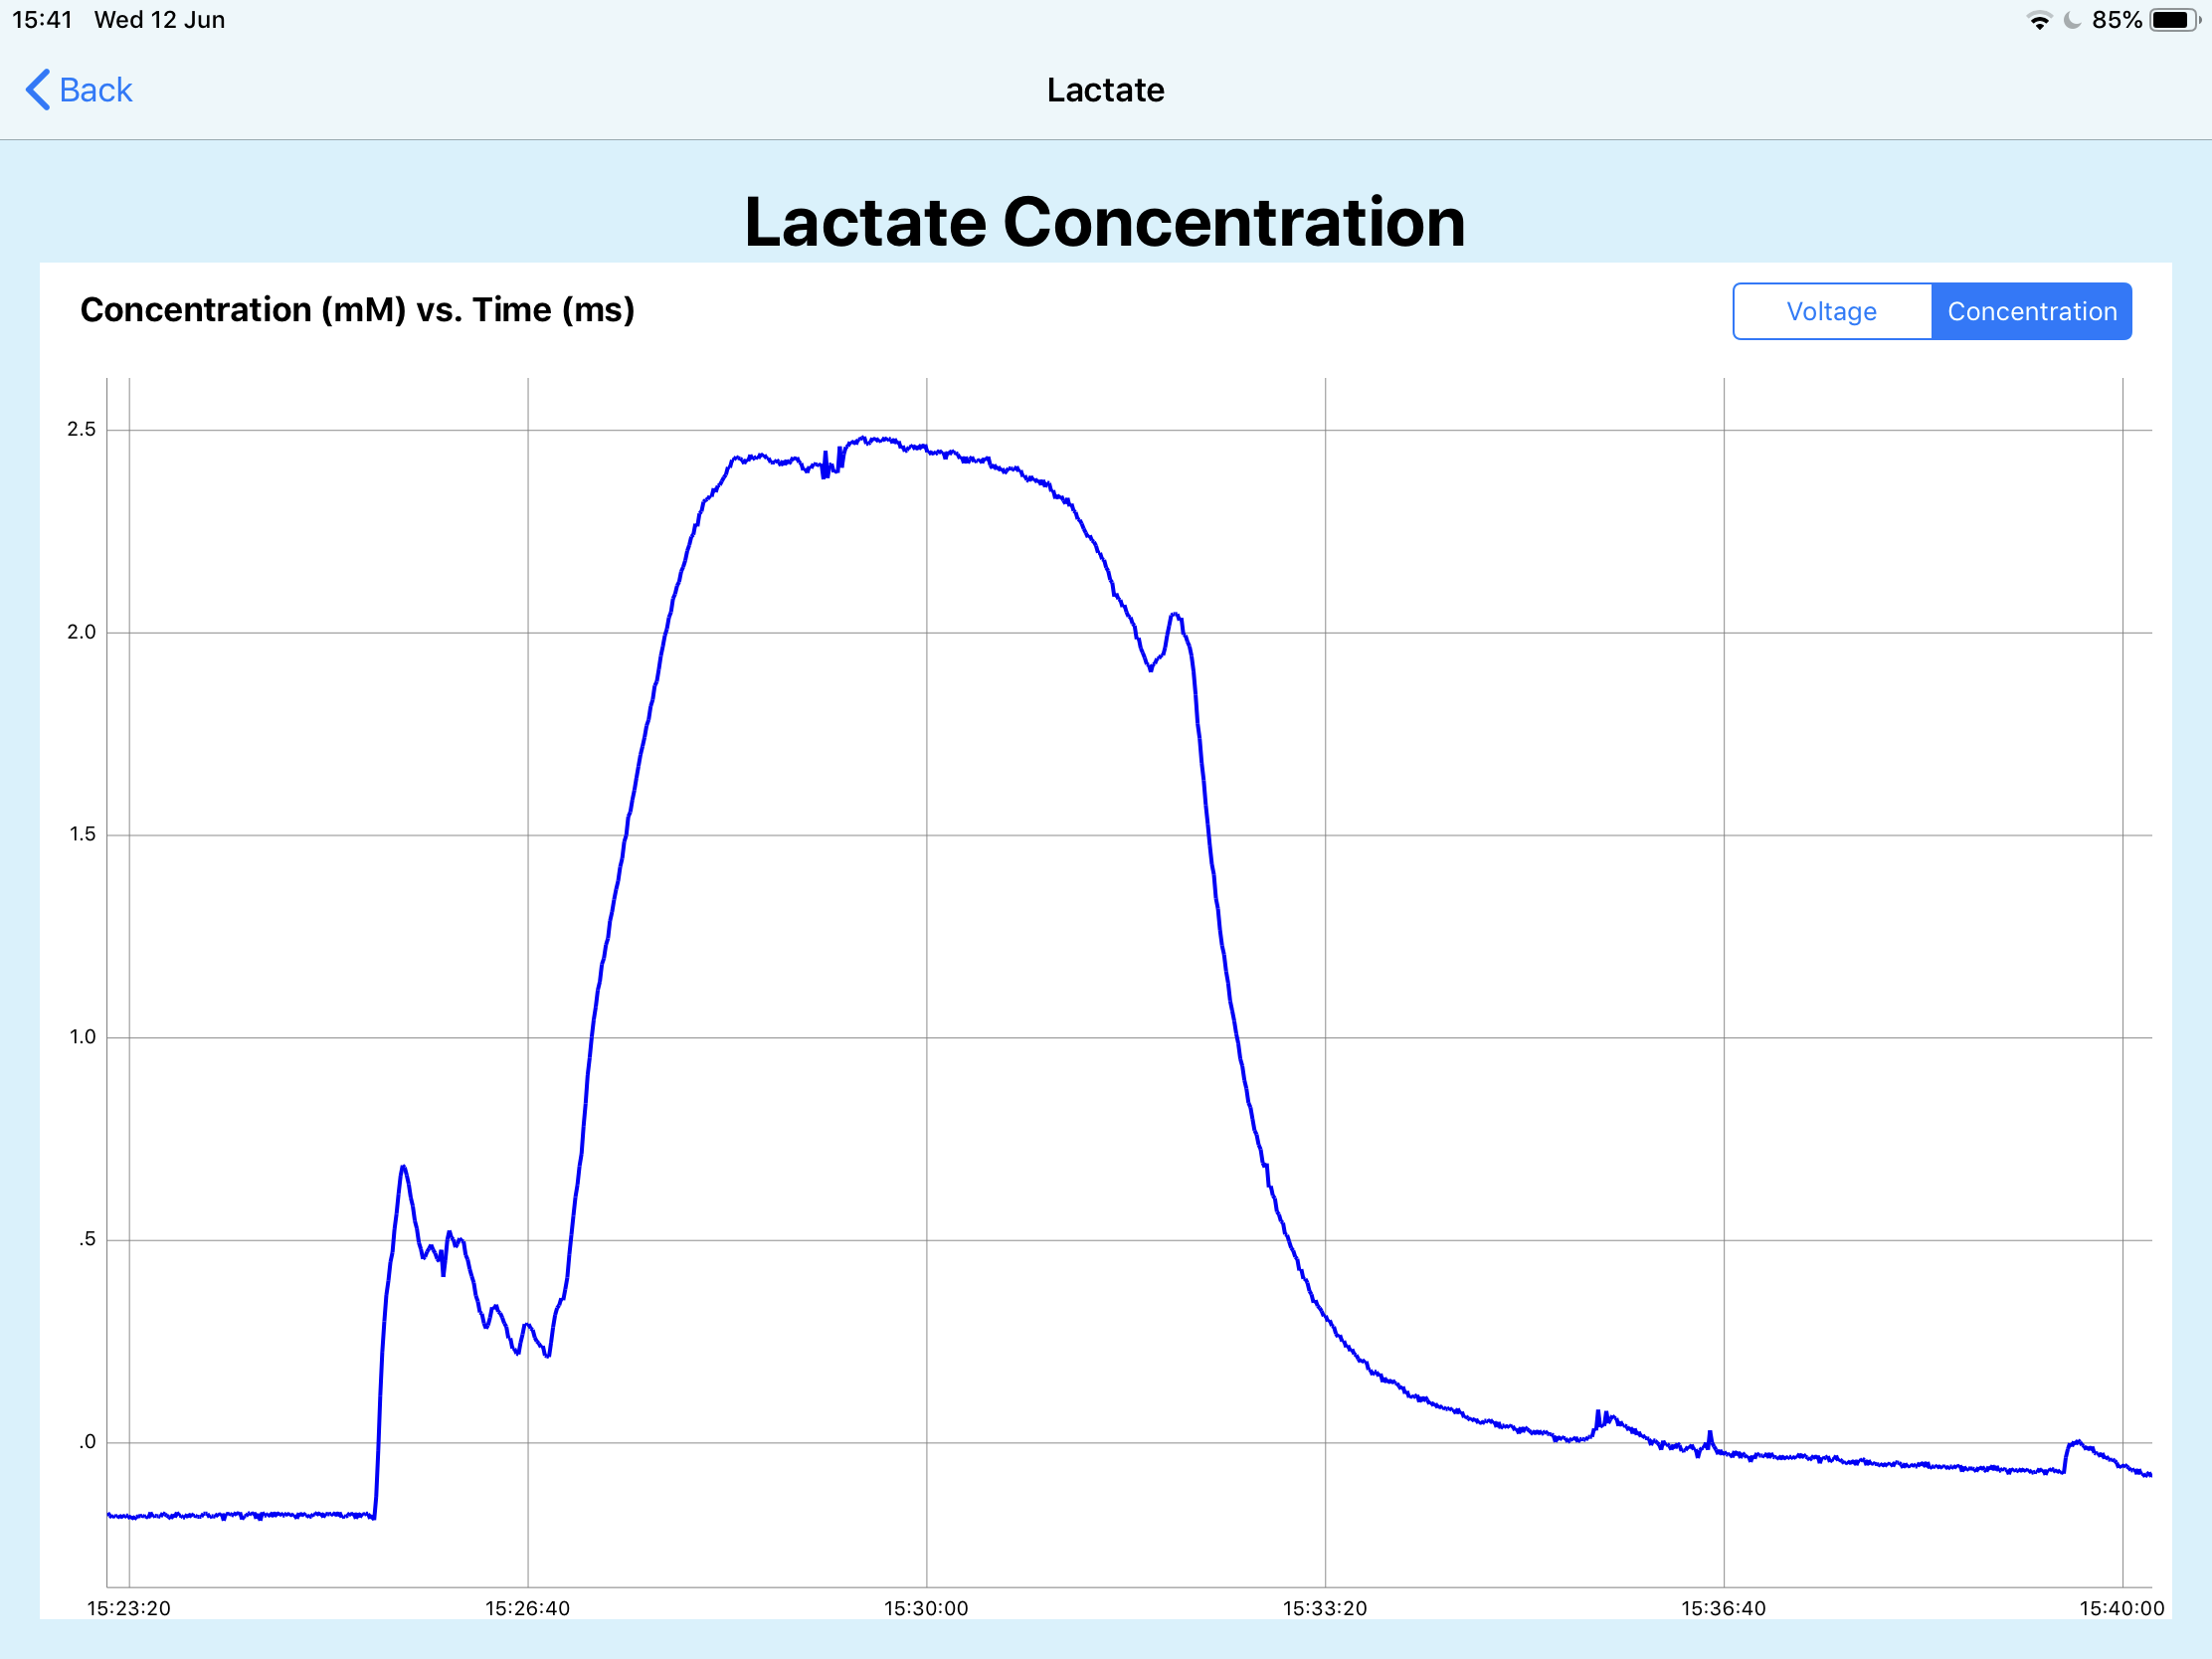
\includegraphics[trim={1.3cm 1.3cm 1.3cm  10cm}, clip, width=.75\textwidth]{./figures/patientsignals/LactateC.PNG}
\bigbreak
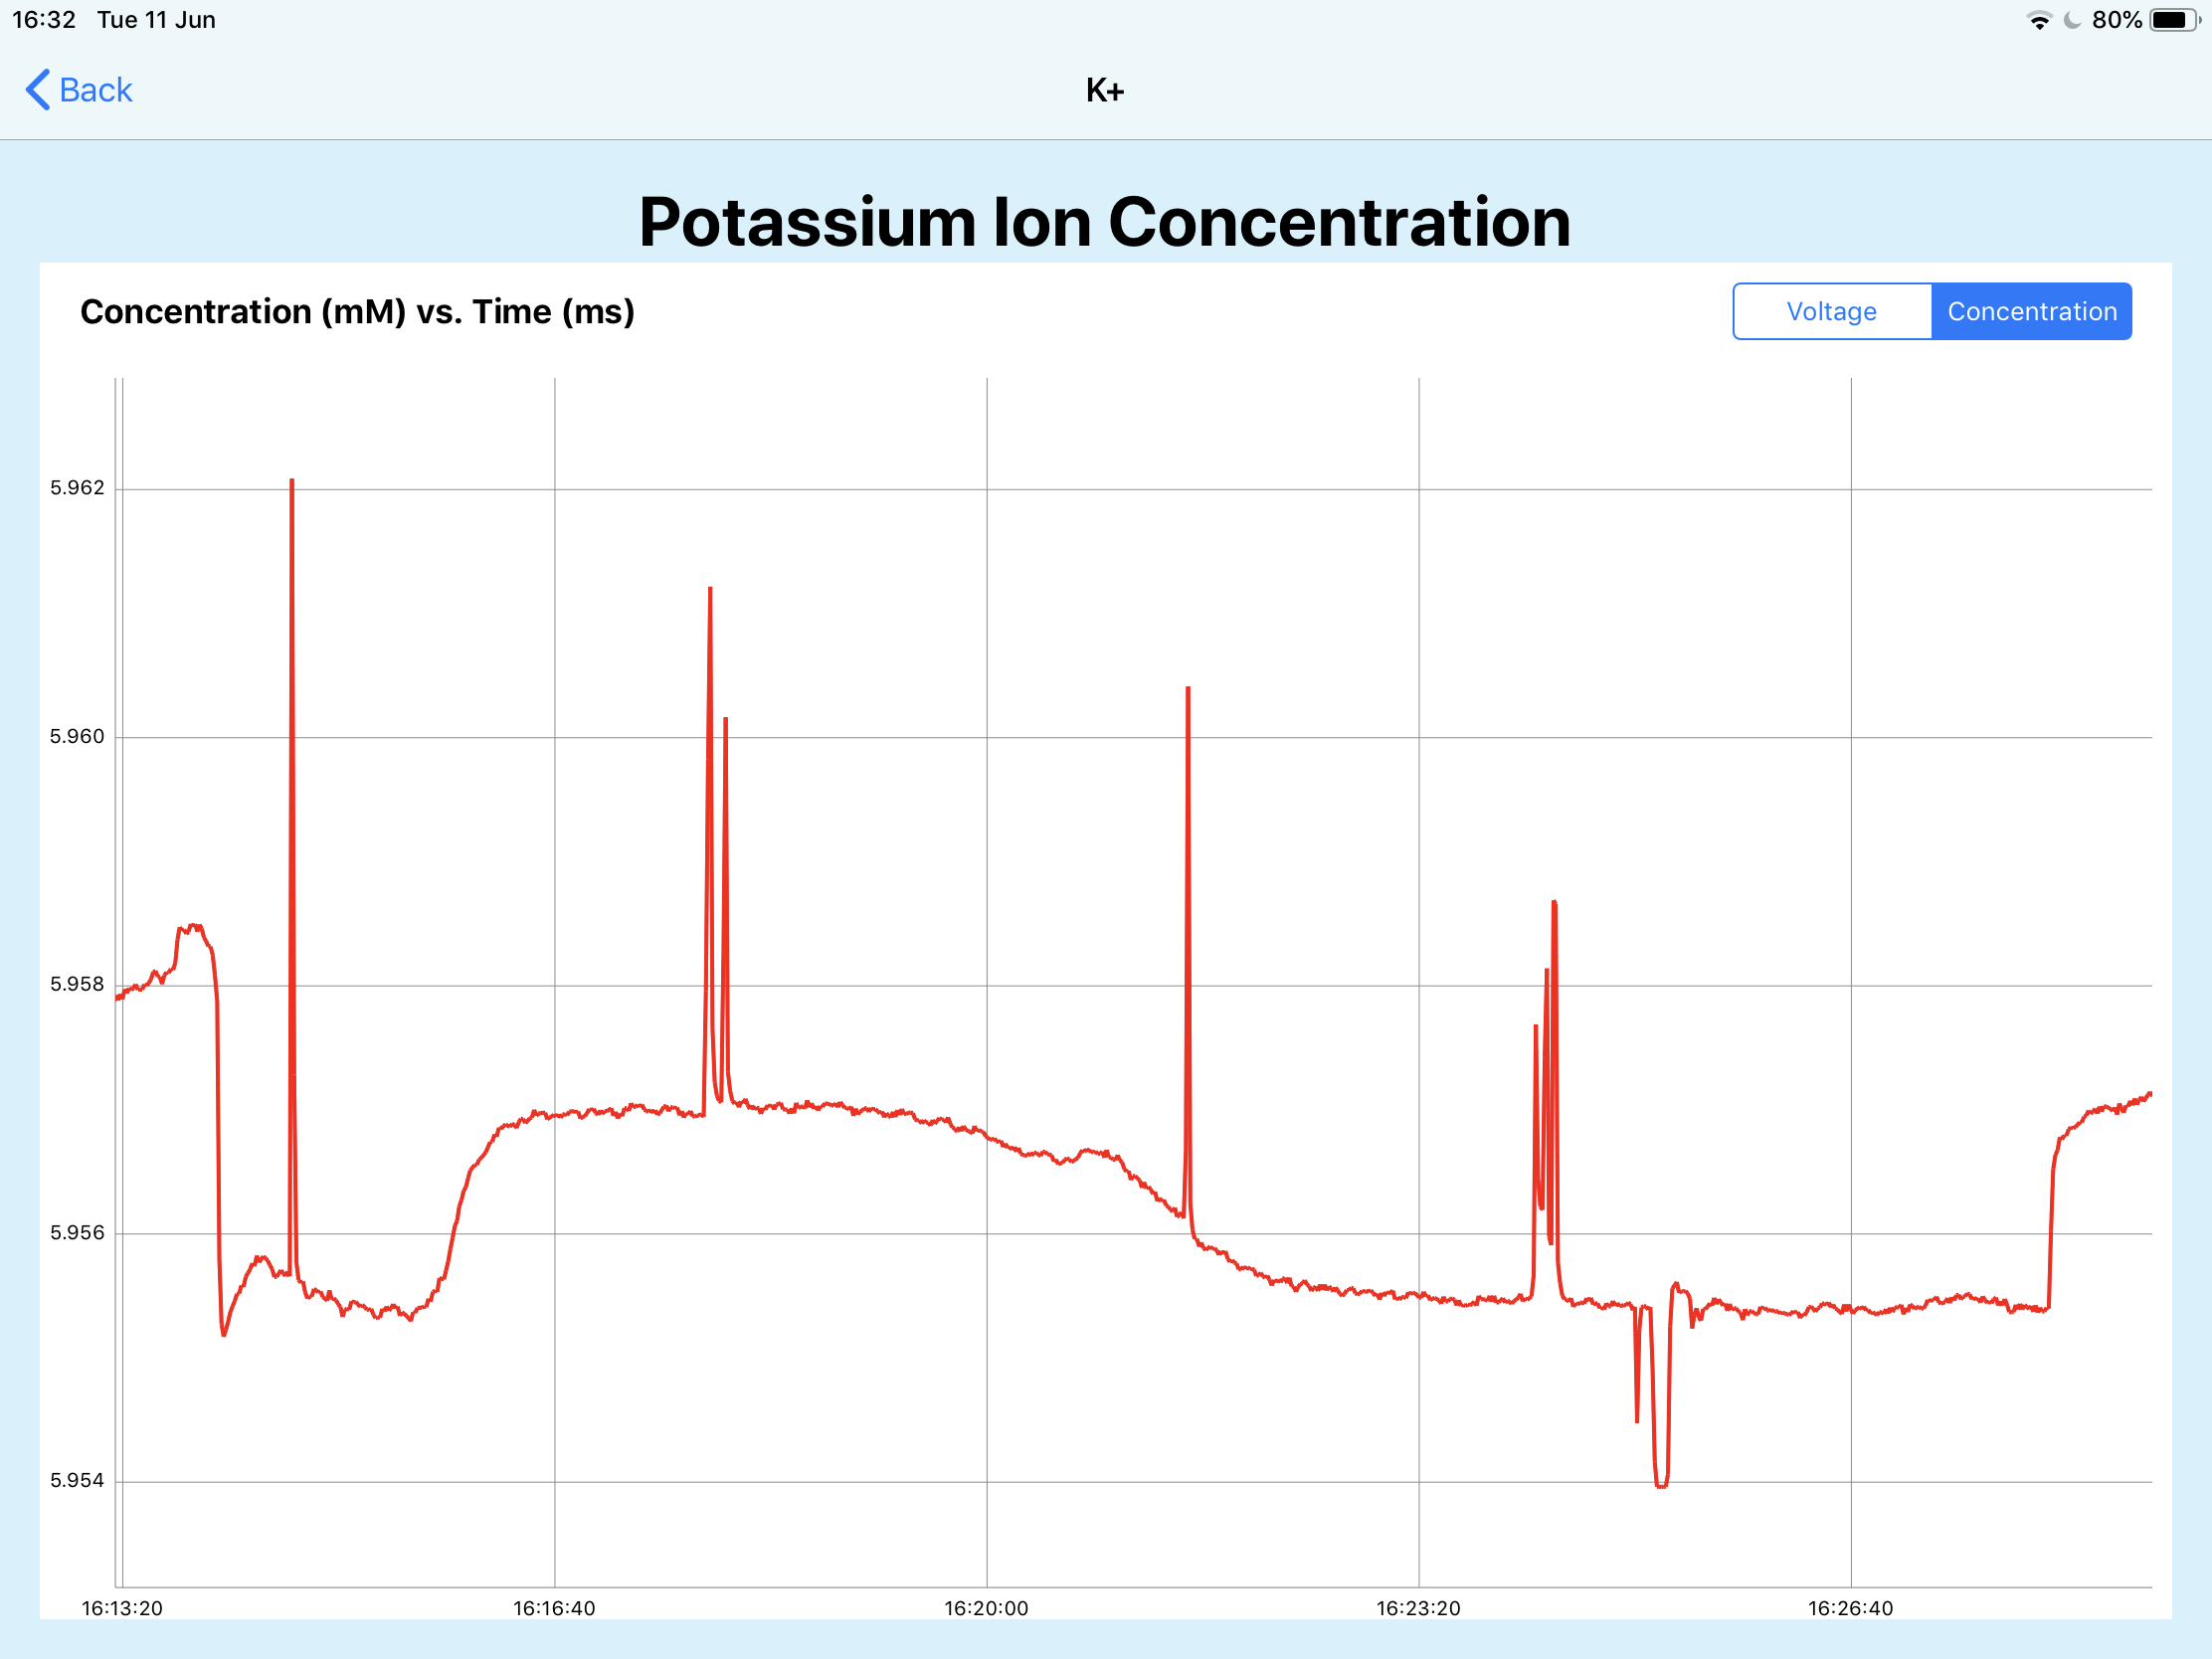
\includegraphics[trim={1.3cm 1.3cm 1.3cm  10cm}, clip, width=.75\textwidth]{./figures/patientsignals/PotassiumC.PNG}
\captionsetup{justification=centering}
\caption{Concentration graphs. Top to bottom: Glucose, Lactate, Potassium.}
\label{fig: test2 conc}
\end{figure}